\section{Introduzione}
Quando si sviluppa un software complesso, diventa necessario pianificare il lavoro da svolgere per creare un prodotto robusto e affidabile.\\
In questa sezione discuteremo dei metodi utilizzati per migliorare lo sviluppo del software, come il sistema di versionamento utilizzato e gli strumenti di pulizia del codice usati per ottenere un prodotto di alta qualità.\\
\section{Versionamento del codice}
È deciso di adottare il sistema di versionamento Git, usando la piattaforma GitHub per ospitare il repository del progetto. Essendo l'applicazione divisa in due blocchi precisi e distinti, il Front end Vue e il Server Backend Spring Boot, sono stati creati due repository per gestirli in modo separato ed evitare maggiori conflitti durante lo sviluppo.\\
Il Team di sviluppo si è coordinato per lavorare su funzionalità separate, in modo da ridurre al minimo i conflitti di merge e facilitare l'integrazione del codice, seguendo le seguenti pratiche:\\
\begin{itemize}
    \item \textbf{Commit Frequency:} Si è deciso di effettuare commit frequenti con messaggi chiari e descrittivi, in modo da tracciare facilmente le modifiche apportate al codice.
    \item \textbf{Code Reviews:} Prima di unire una pull request al branch principale, un altro membro del team esegue una revisione del codice per garantire la qualità e la coerenza con gli standard di codifica stabiliti.
\end{itemize}
\newpage
Nelle figure \ref{fig:resoconto-commit-backend} e \ref{fig:resoconto-commit-frontend} sono riportati i resoconti dei commit effettuati su entrambi i repository durante il periodo di sviluppo.
\begin{figure}[H]
	\centering
	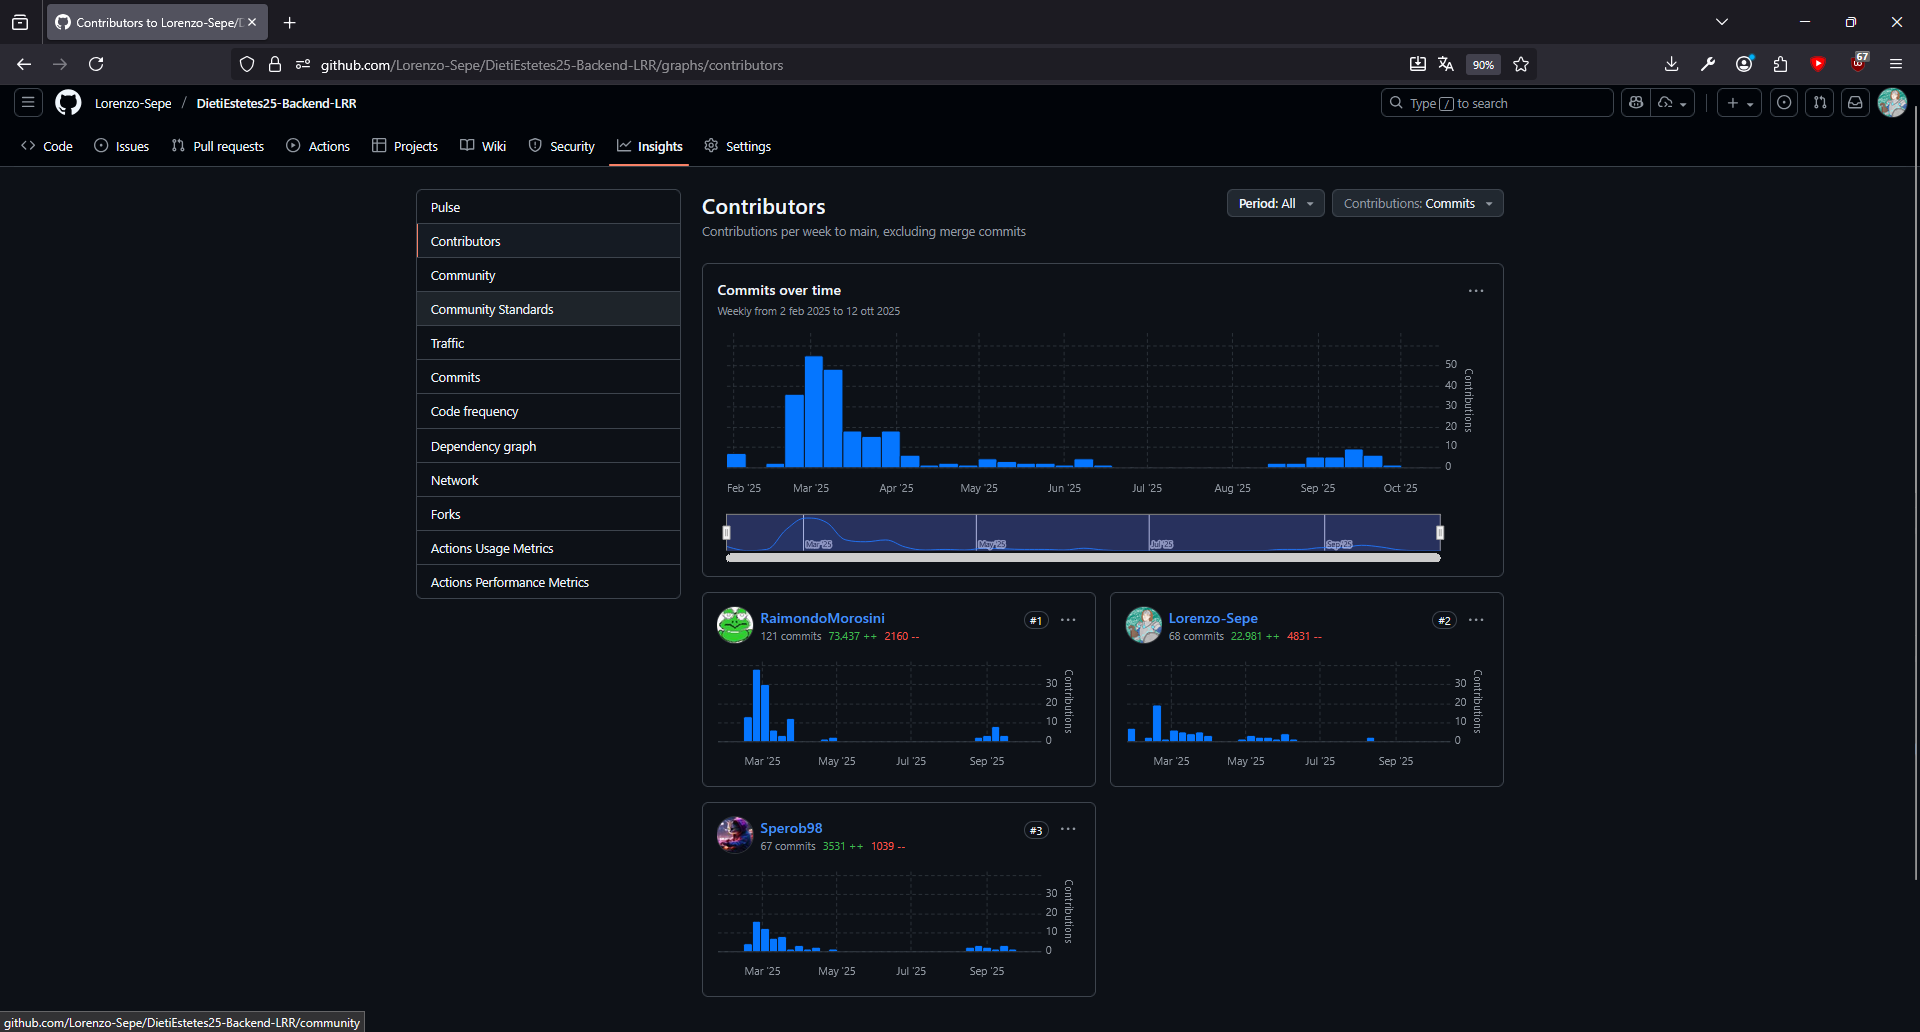
\includegraphics[width=1\linewidth]{"Immagini/Resoconto Commit BE.png"}
	\caption[Resoconto Commit Backend]{}
	\label{fig:resoconto-commit-backend}
\end{figure}
\begin{figure}[H]
	\centering
	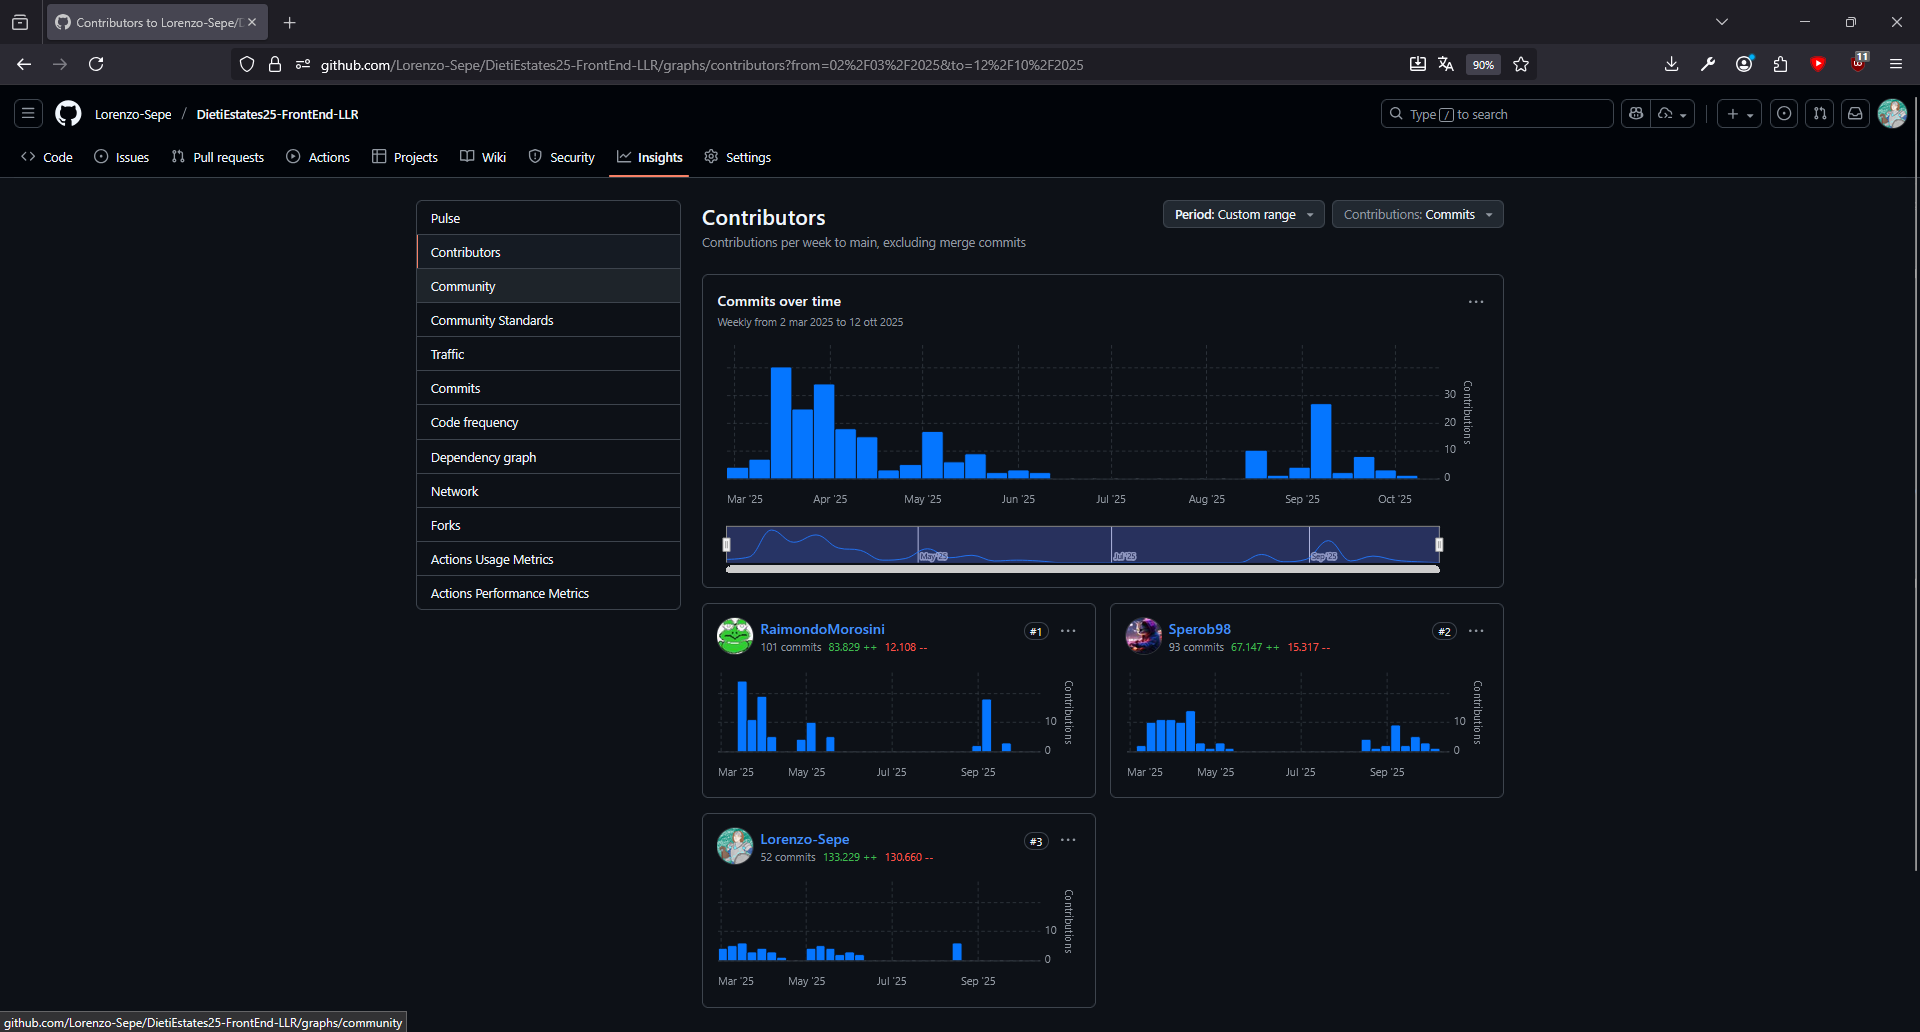
\includegraphics[width=1\linewidth]{"Immagini/Resoconto Commit FE.png"}
	\caption[Resoconto Commit Frontend]{}
	\label{fig:resoconto-commit-frontend}
\end{figure}